% AUTHOR: Ruslan Kiianchuk <ruslan.kiianchuk@gmail.com>

\chapter{Labour protection and safety in emergencies}
\label{sec:labour}

PC users working conditions are analyzed for
their compliance with normative documents on safety engineering  and
sanitation. For retrieving and evaluating the influence of possible dangerous
or harmful production factors an interaction system
``Human--Machine--Environment'' (HME) is developed. Safety measures are
developed as the result of such system analysis.

\section{Analysis of the workplace working conditions}

The administrative building in which the workspace is located situates on the
first floor and has dimensions \sloppy{$6 \times 5.6 \times 3 \, \text{m}$}.

There are three workers in the office that use the following equipment:
\begin{itemize}
    \item Personal computer, 3 pieces;
    \item LCD monitor, 3 pieces.;
    \item Printer;
    \item Monitor.
\end{itemize}
The are also two windows 1.5~m wide and 1.7~m tall and doors 2.1~m tall and
0.9~m wide.
The analysis of the workspace indicates that the office has sufficient area
($6 \, \text{m}^2$) and volume ($20 \, \text{m}^2$) per worker and is compliant
with the sanity standard~\cite{dsanpin} for working with electronic computer
displays (figure~\ref{fig:workstation}).

The ``Human-Machine--Environment'' system (figure~\ref{fig:hme-graph}) is
created with the intention to retrieve possible dangerous and harmful
production factors~\cite{npaop4-12}. The list of H-M-E system connections is
shown in table~\ref{tbl:hme-legend}. Its main elements are:

\begin{description}
    \item[``Human''] --- staff that works in the office (2 workers);
    \item[``Machine''] --- electronic computers;
    \item[``Environment''] --- workspace environment;
    \item[``Product''] --- product of the algebraic cryptanalysis task solution.
\end{description}
Each element of the system contains three functional parts. Thereby the
``Human'' element is split by:
\begin{description}
    \item[$H_1$] --- execution of certain actions targeted on the main task solution;
    \item[$H_2$] --- human as a biological object influencing the environment;
    \item[$H_3$] --- human from the point of view of her psychophysiologic condition. 
\end{description}
The main goal of the ``Machine'' element is influencing the product ---
execution of the primary technological function. Its auxiliary functions are to
generate particular environment parameters and execute emergency surveillance.
\begin{description}
    \item[$M_1$] --- execution of the primary technological function
        (performing computations using SAGE algebra system, construction and
        analysis of algebraic quadratic system that defines the GOST~28147-89
        cipher);
    \item[$M_2$] --- emergency protection support;
    \item[$M_3$] --- influencing the human and the environment.
\end{description}

\begin{figure}[htbp]
	\centering
    %&latex
% Copyright 2011 Zoresvit (c) <zoresvit@gmail.com>
% 
% 
%/

\begin{tikzpicture}
    \tikzstyle{func} = [node distance=7mm, circle, draw=blue!40, fill=blue!20, thick, minimum size = 8mm]
    \tikzstyle{elem} = [circle, draw=green!40, fill=green!20, thick, minimum size = 8mm]
    \tikzstyle{bound} = [node distance=1em]
    \tikzstyle{backfill} = [fill=blue!10, rounded corners]
    \tikzstyle{linkbelow} = [bend right, looseness=0.7]
    \tikzstyle{linkabove} = [bend left, looseness=1.2]
    \tikzstyle{linklabel} = [circle, fill=cyan!10, minimum size=5mm, inner sep=0, draw, above, sloped]

    \node (H1) [node distance=3ex] {\Large $H^1$};
    \node[func] (H11) [below=of H1]  {$H^1_1$};
    \node[func] (H12) [below=of H11] {$H^1_2$};
    \node[func] (H13) [below=of H12] {$H^1_3$};
    \node[bound] (H1bound) [left=of H1] {};

    \node (M1) [node distance=0.7\textwidth, right=of H1]  {\Large $M^1$};
    \node[func] (M11) [below=of M1]  {$M^1_1$};
    \node[func] (M12) [below=of M11] {$M^1_2$};
    \node[func] (M13) [below=of M12] {$M^1_3$};
    \node[bound] (M1bound) [right=of M1] {};

    \node (H2) [node distance=3ex, below=of H13] {\Large $H^2$};
    \node[func] (H21) [below=of H2]  {$H^2_1$};
    \node[func] (H22) [below=of H21] {$H^2_2$}; 
    \node[func] (H23) [below=of H22] {$H^2_3$}; 
    \node[bound] (H2bound) [left=of H2] {};

    \node (M2) [node distance=3ex, below=of M13]  {\Large $M^2$};
    \node[func] (M21) [below=of M2]  {$M^2_1$};
    \node[func] (M22) [below=of M21] {$M^2_2$};
    \node[func] (M23) [below=of M22] {$M^2_3$};
    \node[bound] (M2bound) [right=of M2] {};

    \node (H3) [node distance=3ex, below=of H23] {\Large $H^3$};
    \node[func] (H31) [below=of H3]  {$H^2_1$};
    \node[func] (H32) [below=of H31] {$H^2_2$}; 
    \node[func] (H33) [below=of H32] {$H^2_3$}; 
    \node[bound] (H3bound) [left=of H3] {};

    \node (M3) [node distance=3ex, below=of M23]  {\Large $M^3$};
    \node[func] (M31) [below=of M3]  {$M^2_1$};
    \node[func] (M32) [below=of M31] {$M^2_2$};
    \node[func] (M33) [below=of M32] {$M^2_3$};
    \node[bound] (M3bound) [right=of M3] {};

    \node[elem] (Env) [node distance=0.23\textwidth, minimum size=40mm, right=of H1] {Environment};
    \node[elem] (Prod) [node distance=0.25\textwidth, minimum size=40mm, right=of H32] {Product};


    \foreach \H / \M in {H11/M11, H11/M21, H11/M31, H21/M11, H21/M21, H21/M31, H31/M11, H31/M21, H31/M31}{
    \draw (\H) to [->, linkabove] node[linklabel]{1} (\M);
    }

    \foreach \M / \Prod in {M11/Prod, M21/Prod, M31/Prod}{
    \draw (\M) to [->, linkbelow] node[linklabel]{2} (\Prod) ;
    }

    \foreach \H / \Prod in {H11/Prod, H21/Prod, H31/Prod}{
    \draw (\H) to [<->, linkabove] node[linklabel]{3} (\Prod);
    }

    \foreach \H / \Env in {H12/Env, H22/Env, H32/Env}{
    \draw (\H) to [->, linkbelow] node[linklabel]{4} (\Env);
    }

    \foreach \Env / \H in {Env/H13, Env/H23, Env/H33}{
    \draw (\H) to [<-, linkbelow] node[linklabel]{5} (\Env);
    }

    \foreach \Prod / \H in {Prod/H13, Prod/H23, Prod/H33}{
    \draw (\Prod) to [->, linkbelow] node[linklabel]{6} (\H);
    }

    \foreach \M / \Env in {M13/Env, M23/Env, M33/Env}{
    \draw (\M) to [->, linkabove] node[linklabel]{7} (\Env);
    }

    \foreach \Hact / \Hpsy in {H11/H13, H21/H23, H31/H33}{
    \draw (\Hact) to [->, linkabove] node[linklabel]{8} (\Hpsy);
    }

    \foreach \Hpsy / \Hbio in {H13/H12, H23/H22, H33/H32}{
    \draw (\Hpsy) to [->, linkabove] node[linklabel]{9} (\Hbio);
    }

    \foreach \H / \M in {H11/M13, H21/M23, H31/M33}{
    \draw (\H) to [->, linkabove] node[linklabel]{10} (\M);
    }

    \foreach \Env / \M in {Env/M12, Env/M22, Env/M32}{
    \draw (\Env) to [->, linkbelow] node[linklabel]{11} (\M);
    }

    \draw (H13) to [<->, linkabove] node[linklabel]{12} (H23);
    \draw (H13) to [<->, linkabove] node[linklabel]{12} (H33);
    \draw (M13) to [<->, linkbelow] node[linklabel]{13} (M23);
    \draw (M13) to [<->, linkbelow] node[linklabel]{13} (M33);

    \begin{pgfonlayer}{background}
        \node [backfill, fit= (H1) (H11) (H12) (H13) (H1bound)] {};
        \node [backfill, fit= (M1) (M11) (M12) (M13) (M1bound)] {};
        \node [backfill, fit= (H2) (H21) (H22) (H23) (H2bound)] {};
        \node [backfill, fit= (M2) (M21) (M22) (M23) (M2bound)] {};
        \node [backfill, fit= (H3) (H31) (H32) (H33) (H3bound)] {};
        \node [backfill, fit= (M3) (M31) (M32) (M33) (M3bound)] {};
    \end{pgfonlayer}
\end{tikzpicture}


	\caption{H-M-E system scheme}
	\label{fig:hme-graph}
\end{figure}

\begin{longtable}{|p{0.09\textwidth}|p{0.16\textwidth}|p{0.66\textwidth}|}
\caption{Human--Machine--Enviroment system connections} \label{tbl:hme-legend} \\ \hline
\begin{center} Index \end{center} & Connection direction & \begin{center} Essence of the connections \end{center} \\ \hline
\endfirsthead
\multicolumn{3}{l}{\hfill Proceeding table \thechapter.\arabic{table}}
\endhead
    1 & $H_1 \rightarrow M_1$ & Human controls equipment providing its correct
    functioning (operating on computer using peripheral input devices).  \\ \hline
    2 & $M_1 \rightarrow \text{Prod}$ & Machine influence on the product
    (construction of the cryptographic transformation model, research
    computations). \\ \hline
    3 & $H_1 \leftrightarrow \text{Prod}$ & Human influence on the product and
    backwards (human is the source of ideas that defines needed actions during
    the work and analysis the working process; depending on the project
    complexity and accomplishment success causes mental strain for the
    workers). \\ \hline
    4 & $H_2 \rightarrow \text{Env}$ & Human influence on the environment
    (generation of heat and humidity, temperature increase). \\ \hline
    5 & $\text{Env} \rightarrow H_3$ & Environment influence on human health
    (the psychophysiologic condition working capacity depends on the
    environment conditions). \\ \hline
    6 & $\text{Prod} \rightarrow H_3$ & Product influence on human (complexity
    and execution progress of the primary task influence the human physical
    condition). \\ \hline
    7 & $M_3 \rightarrow \text{Env}$ & Machine influence on environment
    (computer is the source of increased temperature, noise, ionizing and
    electromagnetic emission). \\ \hline
    8 & $H_1 \rightarrow H_3$ & The working activity influences
    human psychophysiologic condition (human psychophysiologic condition
    depends on the success and amount of the completed work). \\ \hline

    9 & $H_3 \rightarrow H_2$ & Influence of psychophysiologic condition on
    human biological processes density (fatigue, irritability, euphoria). \\ \hline 
    10 & $H_1 \rightarrow M_3$ & 
    Human control of the machine influence on environment (normalization of
    harmful emission, humidity and temperature control). \\ \hline
    11 & $\text{Env} \rightarrow M_2$ & Environment influence on emergency
    protection abilities (unfavourable environment parameters may lead to
    insufficient emergency protection). \\ \hline
    12 & $H^*_3 \leftrightarrow H^*_3$ & Reciprocal influence of each human's
    psychophysiologic conditions. \\ \hline
    13 & $M^*_1 \leftrightarrow M^*_1$ & Mutual influence of machine side
    emissions. \\ \hline
\end{longtable}

Based on the analysed connections harmful and dangerous production factors may
be retrieved according to~\cite{gost003}. The following harmful factors are
found:
\begin{itemize}
    \item physical: 
        \begin{enumerate}
            \item increased electromagnetic emission;
            \item increased equipment surface temperature;
            \item reduced air humidity;
        \end{enumerate}
    \item chemical: absent;
    \item biological: absent;
    \item psychophysiologic: 
        \begin{enumerate}
            \item mental overstress;
            \item overstress of analyzers.
        \end{enumerate}
\end{itemize}
Reduced air humidity is the dominant harmful factor.


\begin{longtable}{|p{0.35\textwidth}|p{0.09\textwidth}|p{0.09\textwidth}|c|c|c|p{0.12\textwidth}|}
\caption{Evaluation for factors of working environment} \label{tbl:hme-legend} \\ \hline
\begin{center} Factors \end{center} & \begin{center}Norm\end{center} & \begin{center} Fact \end{center} & 1 st. & 2 st. & 3 st. & duration, \% for working shift\\ \hline
\endfirsthead
\multicolumn{7}{l}{\hfill Proceeding table \thechapter.\arabic{table}}
\endhead
Noise & 50 & 49 &  &  &  & 93 \\ \hline
Non-ionising radiation & & &  &  &  & \\ \hline 
5~Hz -- 2~kHz & 25 & less 25 &  &  & & 93 \\ \hline 
2~kHz -- 400~kHz & 2.5 & less 2.5 &  &  & & 93 \\ \hline 
X-ray radiation & less 100 & 14 &  &  & & 93 \\ \hline 
Micro climate & & &  &  & & \\ \hline 
Air temp. & 22-24\newline 23-25 & 31.5 &  & + & &  100 \\ \hline 
Air movement & 0.1\newline 0.1 & less 0.1 &  &  & &  100 \\ \hline 
Relative humidity& 60-40\newline 60-40 & less 65 &  &  & &  100 \\ \hline 
Light & & &  &  & &  \\ \hline 
Natural & 1.2 & 1.2 &  &  & & 93 \\ \hline 
Artificial light & 200-500 & 370 &  &  & & 93 \\ \hline 
Work intensity & & &  &  & & \\ \hline 
Attention & & &  &  & & \\ \hline 
Duration of concentration & 25-50 & 48 &  &  & & 48 \\ \hline 
Signals density & 75-175 & less 75 &  &  & & 93 \\ \hline 
Density of analyzers & & &  &  & & \\ \hline 
Eyesight & 2-3 & 3 &  &  & & 93 \\ \hline 
Hearing & unders. words 70--90~\% & 3 &  &  & & 93 \\ \hline 
 Emot. \& Intel. density & Resp. for func. quality & Resp. for perform.  tasks &  &  & & 93 \\ \hline 
Repetitive routines &  & &  &  & & \\ \hline 
Repetitive tasks & 100-25 & 100-25 &  &  & & 93 \\ \hline 
Observ. process & 46-80 & 80 &  &  & & 80 \\ \hline 
Shifts & & day &  &  & & \\ \hline 
No. fuctors & 9 &  &  &  & & \\ \hline 
\end{longtable}

The exceeding factor is air temperature. During the working process of the staff
because of heat emission the temperature raises to $31.5^\circ$~C (3 cl. 2 st.)
and is harmful for health of the staff. For normalizing the air temperature
conditioning system must be set up with precomputed parameters.

\section{Industrial security in production building}
Considering the electrical equipment located in the office, organizational and
technical countermeasures for protecting workers' safety need to be applied.
The workspace belongs to the class of increased fire threat according
to~\cite{npaop1-21}.

The building power supply is three-phased four-wired electric network with
dead-earthed neutral, alternating current, 50~Hz frequency and $380/220$~V
voltage. Neutral grounding of the equipment is done for providing electrical
security according to~\cite{gost030}. The current threshold for automatic
overload control exceeds the maximum equipment current consumption 5 times.
Triggering time of the overload controller does not exceed 0.2~s.

\section{Labour health at the workplace}

According to~\cite{dsanpin} microclimate the standards for given room that
corresponds to power inputs category \verb+Ia+ are shown in
table~\ref{tbl:aero-req}.

\begin{table}[htbp]
    \centering
    \caption{Microclimate standards}
    \label{tbl:aero-req}
    \begin{tabular}{|l|l|l|l|}
        \hline
        Season & Air temp., $^\circ$C & Rel. humid., \% & Air movement, m/s\\ \hline
       Cold & 22-24 & 60-40 & 0.1 \\ \hline
       Hot & 23-25 & 60-40 & 0.1 \\ \hline
    \end{tabular}
\end{table}

For providing the expected climate conditions an air conditioning system needs
to be set up in the room. For computing the required parameters of air
conditioning system on needs to compute the heat coming into the room from
sunlight, artificial light, humans and equipment.

Sources of heat are split into:
\begin{description}
    \item[$Q_1$] --- heating from environment;
    \item[$Q_2$] --- heating from humans;
    \item[$Q_3$] --- heating from equipment.
\end{description}
Overall heating is computed by the formula $Q = Q_1 + Q_2 + Q_3$. Input heat
from environment is computed as follows:
\begin{equation}
Q_1 = (S \cdot h \cdot q) / 1000, 
\end{equation}

where $S$ -- room area, $h$ -- height of the room, $q$ -- load unit (when mean
lightning is 35~W/$m^2$). Heat income from humans is estimated as 0.13~kW. Heat
income from a PC is estimated in 0.3~kW. Heating income from printer is
neglectful. According to these factors the overall heating input equals:
\begin{equation}
Q = Q_1 + Q_2 + Q_3 = (33.6 \cdot 3 \cdot 35) / 1000 + 0.13 \cdot 3 + 0.3 \cdot
3 = 4.87\text{~kW}\enspace.
\end{equation}

Power of conditioning system must be in the range $-5\%$ -- $+15\%$ from
computed power $Q$. So in order to provide the required climate conditions in
the room the conditioning system with power 4.87~kW must be installed. According
to conditioning power catalogue the most satisfying model is Panasonic
CS-E18MKDW with power of 5~kW.

\begin{figure}[htbp]
    \centering
    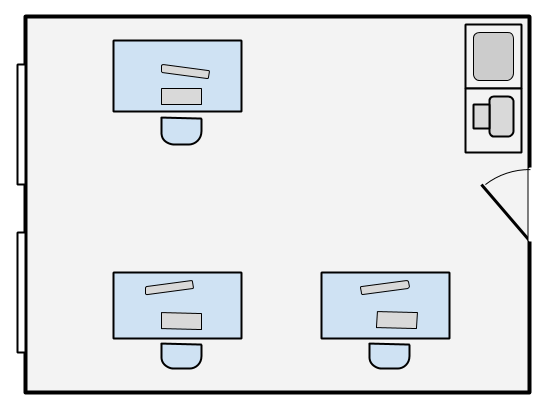
\includegraphics[scale=0.5]{images/workstation}
    \caption{Workstations location in the room}
    \label{fig:workstation}
\end{figure}

\section{Fire safety of the production building}
Solid ignitable materials are used in the room, the building has brick walls
and armoured concrete floor. Therefore the building belongs to 2-nd fire
resistance ratio according to~\cite{dbn_b11}, production belongs to category B
of flammability and explosion risk according to~\cite{napb002}.

Pursuant to~NAPB B.03.001-2004 the building must have two fire extinguishers with
up to 6~kg of reactant or one fire extinguisher with at least 8~kg of reactant.
Any type of fire extinguishers fits for the category B building.

Evacuation plans that are located in every room and in corridors allow to
efficiently leave the building in case of fire through the main exit of 
 $1.9 \, \text{m}$ hight and $1.2 \, \text{m}$ wide. Two employees work at the
 office with area of $25 \, \text{m}^2$. Therefore no extra emergency exit is
 needed. The fire and explosion safety requirements are satisfied.


